%%%%%%%%%%%%%%%%%%%%%%%%%%%%%%%%%%%%%%%%%%%%%%%%%%%%%%%%%%%%%%%

% Set up document

\documentclass{beamer}
% For themese see https://hartwork.org/beamer-theme-matrix/
%\usetheme{Warsaw}
\usecolortheme{beetle}
\setbeamersize{text margin left=5mm,text margin right=5mm}

% Used to create a section slide between section
\AtBeginSection[]{
  \begin{frame}
  \vfill
  \centering
  \begin{beamercolorbox}[sep=8pt,center,shadow=true,rounded=true]{title}
    \usebeamerfont{title}\insertsectionhead\par%
  \end{beamercolorbox}
  \vfill
  \end{frame}
}

% Remove default navigation symbols and add just  page number
\setbeamertemplate{navigation symbols}{} % Clear default navigation
\addtobeamertemplate{navigation symbols}{}{%
    \usebeamerfont{footline}%
    \usebeamercolor[fg]{footline}%
    \hspace{1em}%
    \insertframenumber/\inserttotalframenumber
}


%%%%%%%%%%%%%%%%%%%%%%%%%%%%%%%%%%%%%%%%%%%%%%%%%%%%%%%%%%%%%%%

% Title page text

\title{Stroke Audit Machine Learning (SAMueL)}
\subtitle{Learnings from explainable machine learning: Comparing thrombolysis decisions between hospitals}


\author{Kerry Pearn\inst{1}, Michael Allen\inst{1,3}, Anna Laws\inst{1}, Richard Everson\inst{3}, Martin James\inst{1,2} }
\institute{\inst{1}University of Exeter Medical School \inst{2}Royal Devon University Healthcare NHS Foundation Trust \inst{3}University of Exeter Institute of Data Science and Artificial Intelligence}

%\institute{Overleaf}
\date{January 2023}


\begin{document}

%%%%%%%%%%%%%%%%%%%%%%%%%%%%%%%%%%%%%%%%%%%%%%%%%%%%%%%%%%%%%%%

%\frame{\titlepage}

\begin{frame}
\titlepage
\end{frame}

%%%%%%%%%%%%%%%%%%%%%%%%%%%%%%%%%%%%%%%%%%%%%%%%%%%%%%%%%%%%%%%


\begin{frame}
\frametitle{Thrombolysis rates vary .... a lot}
Here we show the range of thrombolysis use across the 132 acute stroke centres in England and Wales.
\begin{center}
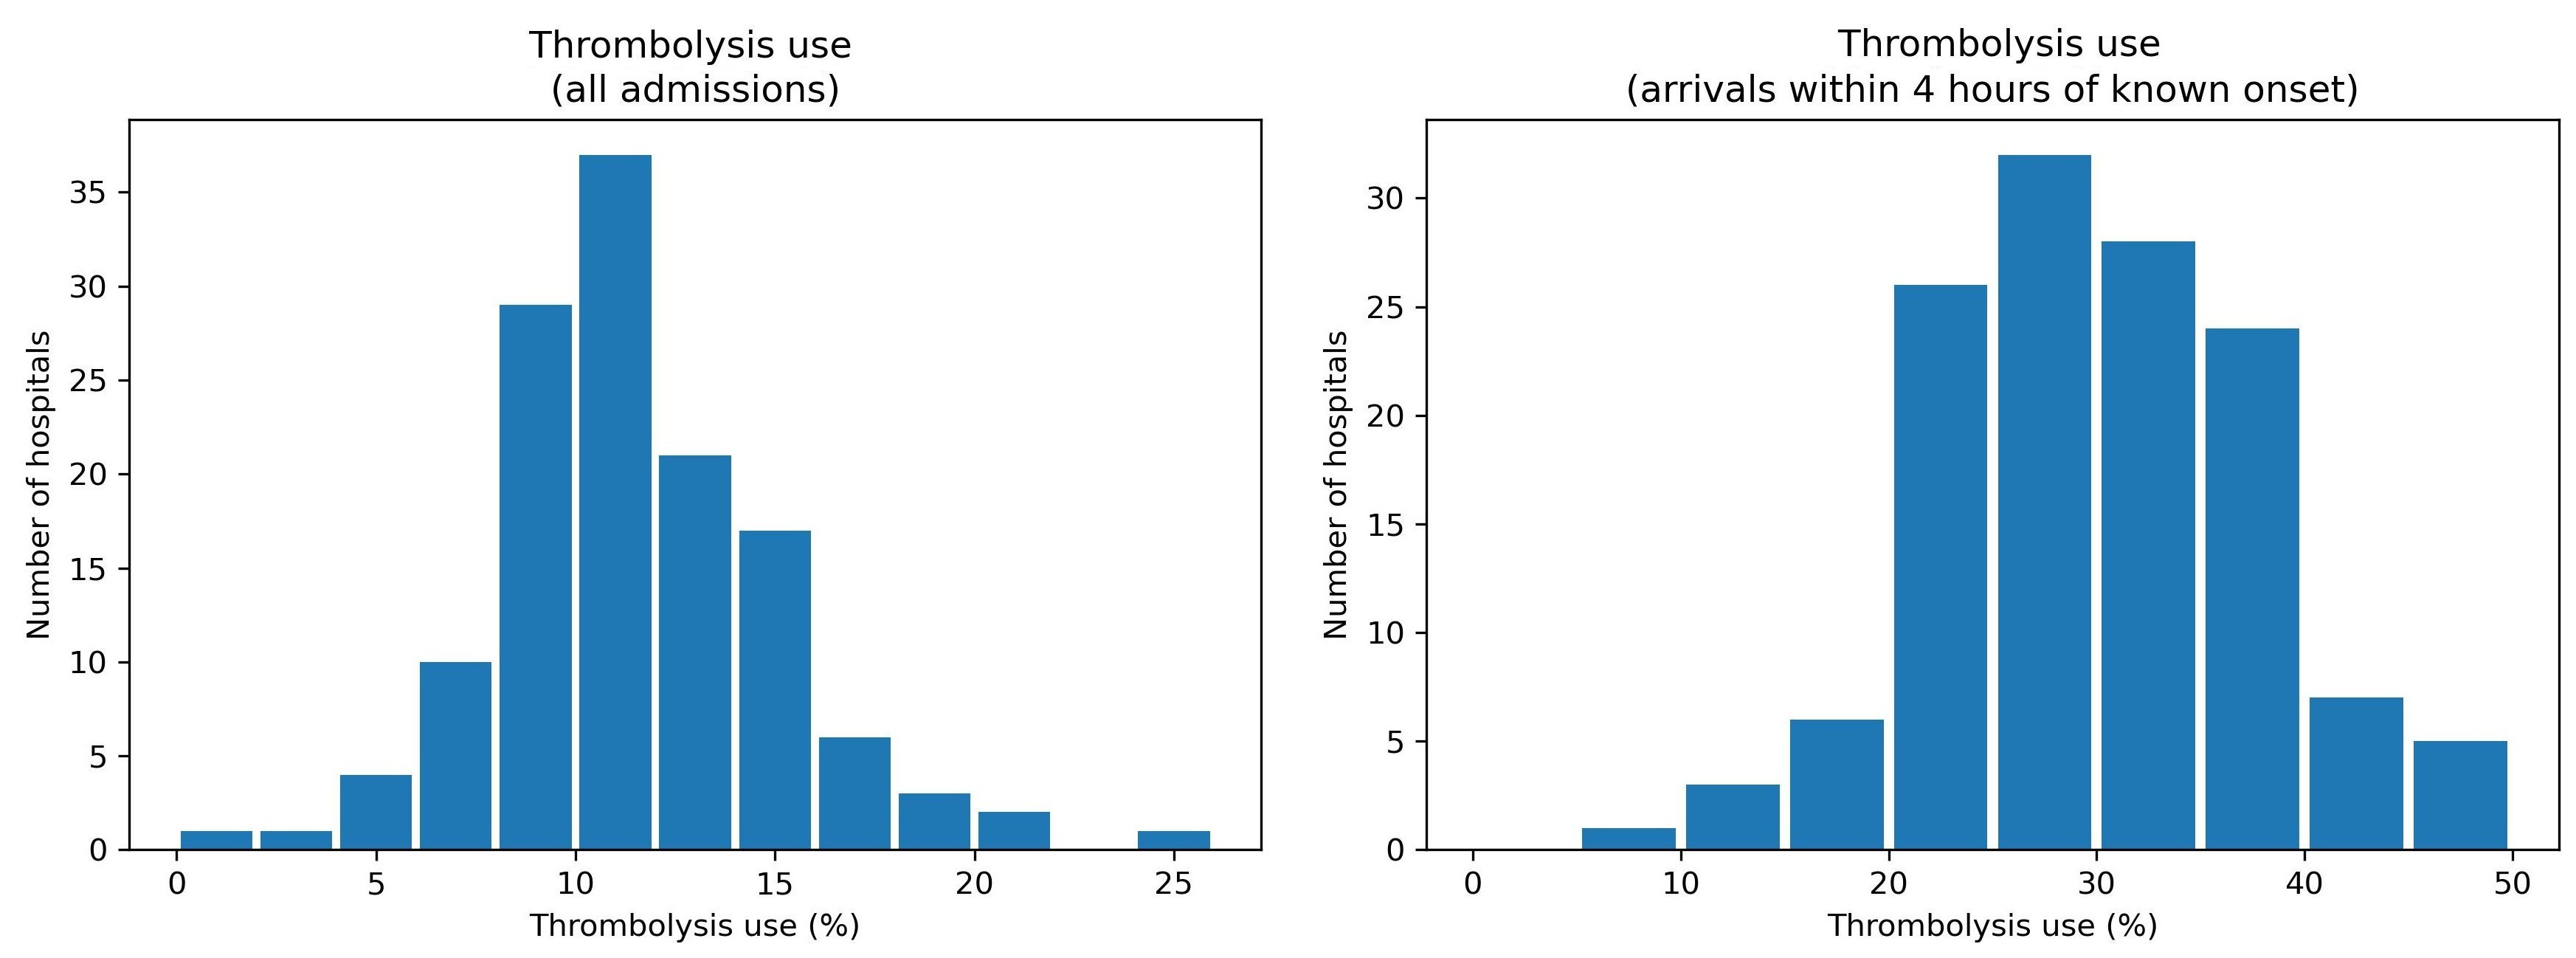
\includegraphics[width=1.0\textwidth]{./images/thrombolysis_hist}
\end{center}

How much of this variation is due to differences in decisions hospitals make on who they would give thrombolysis to?
\end{frame}

%%%%%%%%%%%%%%%%%%%%%%%%%%%%%%%%%%%%%%%%%%%%%%%%%%%%%%%%%%%%%%%

\begin{frame}
\frametitle{Breaking down the emergency stroke pathway into key steps}
\begin{center}
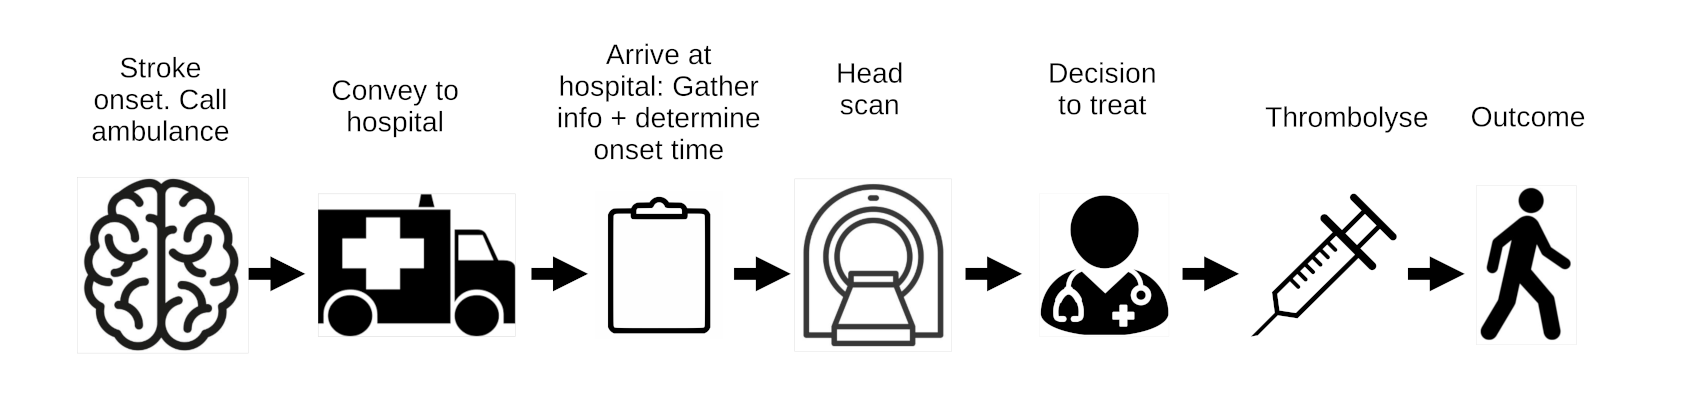
\includegraphics[width=1.0\textwidth]{./images/pathway}
\end{center}
We can model key changes to pathway:
\begin{small}
\begin{itemize}
    \item What if the pathway were faster?
    \item What if hospital determined the stroke onset time in more patients?
    \item What if clinical decision-making was like that of \emph{benchmark} hospitals? (Predict what treatment a patient would receive at other hospitals).
\end{itemize}
\end{small}
\footnotesize{We model these changes with a hospital's own patient population, to allow for inter-hospital variation in patient population characteristics.}
\end{frame}

%%%%%%%%%%%%%%%%%%%%%%%%%%%%%%%%%%%%%%%%%%%%%%%%%%%%%%%%%%%%%%%

\begin{frame}
\frametitle{Machine learning overview}
\begin{center}
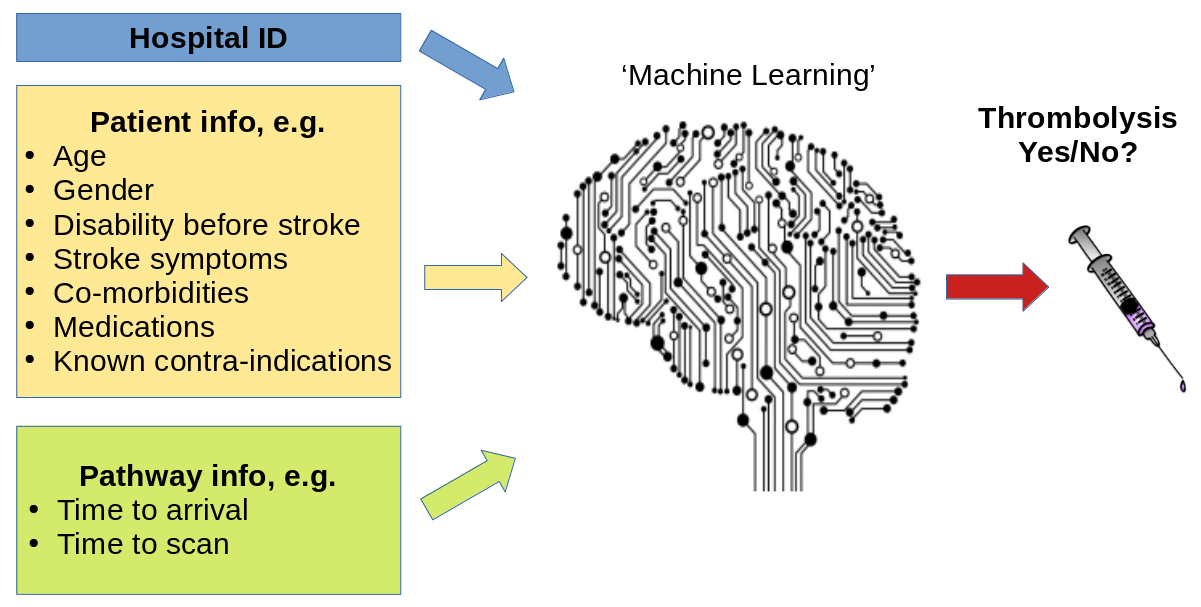
\includegraphics[width=0.90\textwidth]{./images/ml_model_high_level}
\end{center}


Machine learning (and nearly all \emph{artificial intelligence}) is based on the simple principle of recognising similarity to what has been seen before.
\vspace{3mm}

We accessed 240,000 emergency stroke admissions in England and Wales over three years.
\end{frame}


%%%%%%%%%%%%%%%%%%%%%%%%%%%%%%%%%%%%%%%%%%%%%%%%%%%%%%%%%%%%%%%

\begin{frame}
\frametitle{A \emph{Black Box} model}
When we don't know how a model is making predictions we call it a \emph{Black Box} model.
\vspace{4mm}
\begin{center}
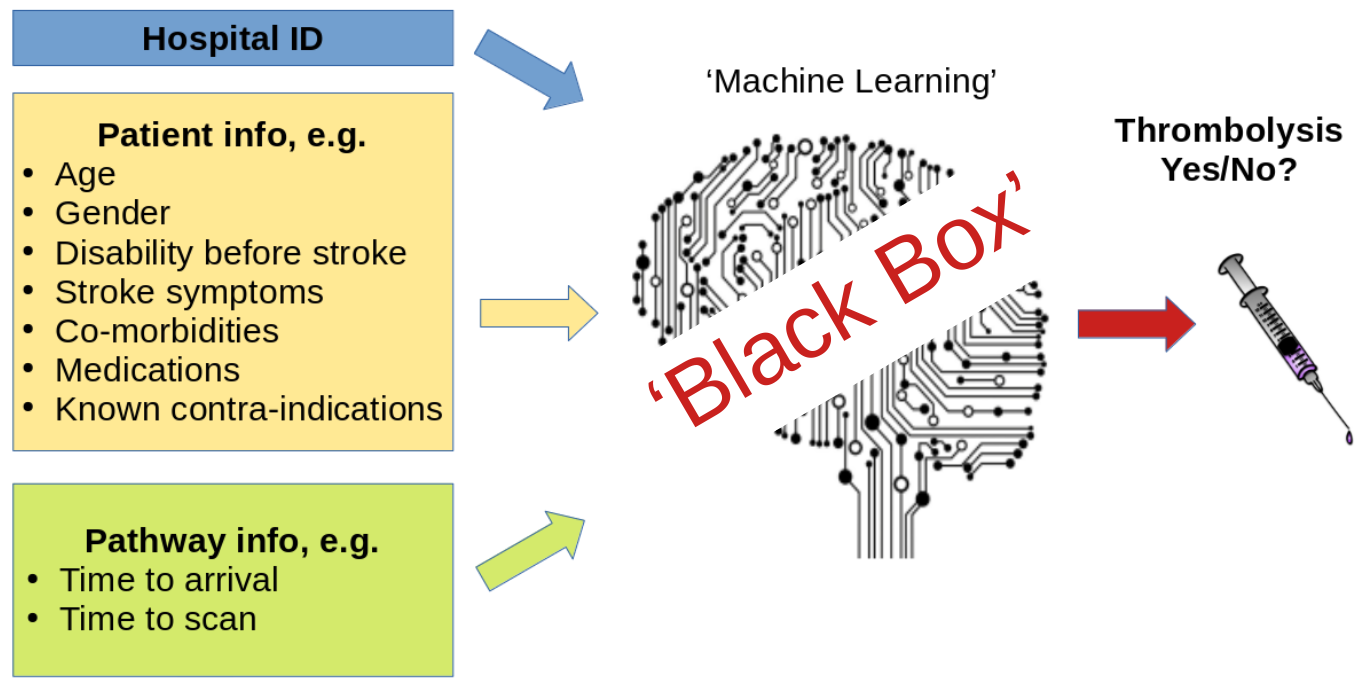
\includegraphics[width=0.90\textwidth]{./images/black_box}
\end{center}
\end{frame}


%%%%%%%%%%%%%%%%%%%%%%%%%%%%%%%%%%%%%%%%%%%%%%%%%%%%%%%%%%%%%%%

\begin{frame}
\frametitle{Simplifying our model}

In order to simplify the model, to make it easier to explain, we reduced the number of patient features from 60 to 10, with almost no loss of model accuracy.

\small
\begin{itemize}
    \item \emph{Arrival-to-scan time}: Time from arrival at hospital to scan (mins)
    \item \emph{Infarction}: Stroke type (infarction or haemorrhage)
    \item \emph{Stroke severity}: Stroke severity (NIHSS) on arrival (ranges from 0 to 42)
    \item \emph{Precise onset time}: Onset time is known precisely
    \item \emph{Prior disability level}: Disability level (modified Rankin Scale) before stroke
    \item \emph{Stroke team}: Stroke team attended
    \item \emph{Use of AF anticoagulants}: Use of atrial fibrillation anticoagulant
    \item \emph{Onset-to-arrival time}: Time from onset of stroke to arrival at hospital
    \item \emph{Onset during sleep}: Did stroke occur in sleep?
    \item \emph{Age}: Age (as middle of 5 year age bands)
\end{itemize}
\end{frame}

%%%%%%%%%%%%%%%%%%%%%%%%%%%%%%%%%%%%%%%%%%%%%%%%%%%%%%%%%%%%%%%

\begin{frame}
\frametitle{SHAP values - looking into the \emph{Black Box}}

SHAP (SHapley Additive exPlanations) values show us the contribution of each patient feature, even in a \emph{Black Box} model.
\vspace{2mm}
These are found by running predictions lots of times with only part of the data for each patient available each time.


\begin{center}
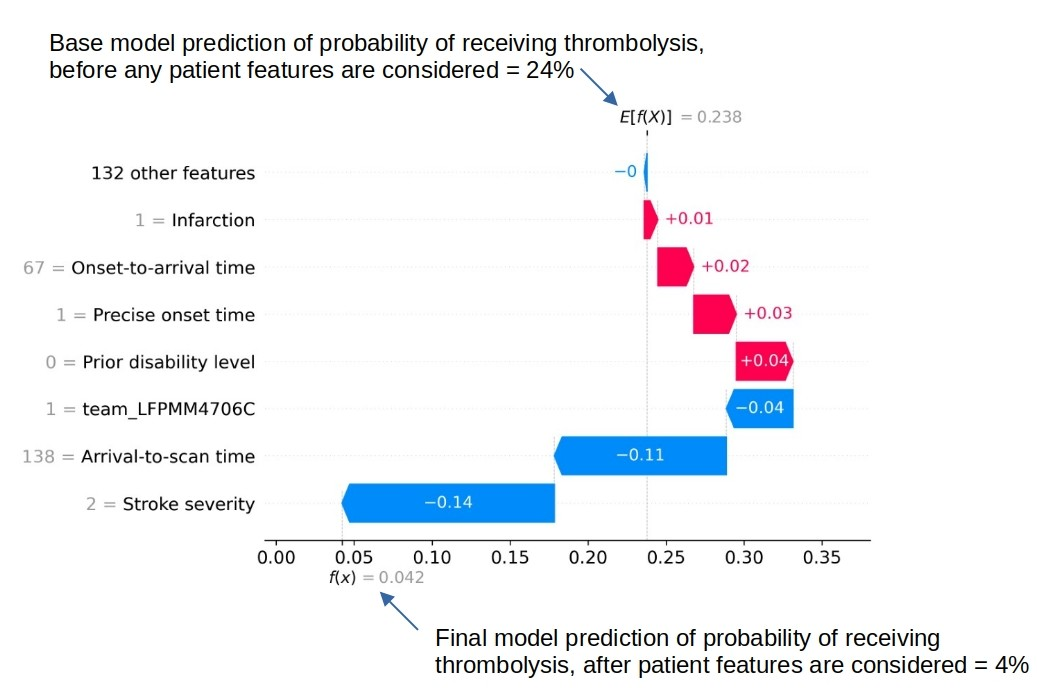
\includegraphics[width=0.75\textwidth]{./images/xgb_waterfall_low_probability_2}
\end{center}
\end{frame}

\begin{frame}
\frametitle{What general patterns did we see?}

The  model revealed that the odds of receiving thrombolysis:
\vspace{1mm}
\begin{itemize}
    \item Reduced 20 fold over the first 100 minutes of arrival-to-scan time
    \item Varied 30 fold depending on stroke severity, with lowest thrombolysis use at low or very high stroke severities
    \item Reduced 3 fold when the stroke onset time was not precisely known
    \item Fell 5 fold with increasing pre-stroke disability
    \item Varied 15 fold between hospitals
\end{itemize}

\vspace{2mm}

The majority of the variation in thrombolysis use between hospitals may be explained by differences in the hospitals’ willingness to use the treatment, rather than the characteristics of the patients they treated.

\vspace{2mm}

Compared with hospitals with higher thrombolysis use, hospitals with lower use were particularly less likely to give thrombolysis to patients with milder strokes, prior disability, or patients with imprecise onset time.

\end{frame}

%%%%%%%%%%%%%%%%%%%%%%%%%%%%%%%%%%%%%%%%%%%%%%%%%%%%%%%%%%%%%%%

\begin{frame}
\frametitle{Viewing the SHAP results}
The previous observations on what affects the odds of receiving thrombolysis, came from these SHAP plots.
\begin{center}
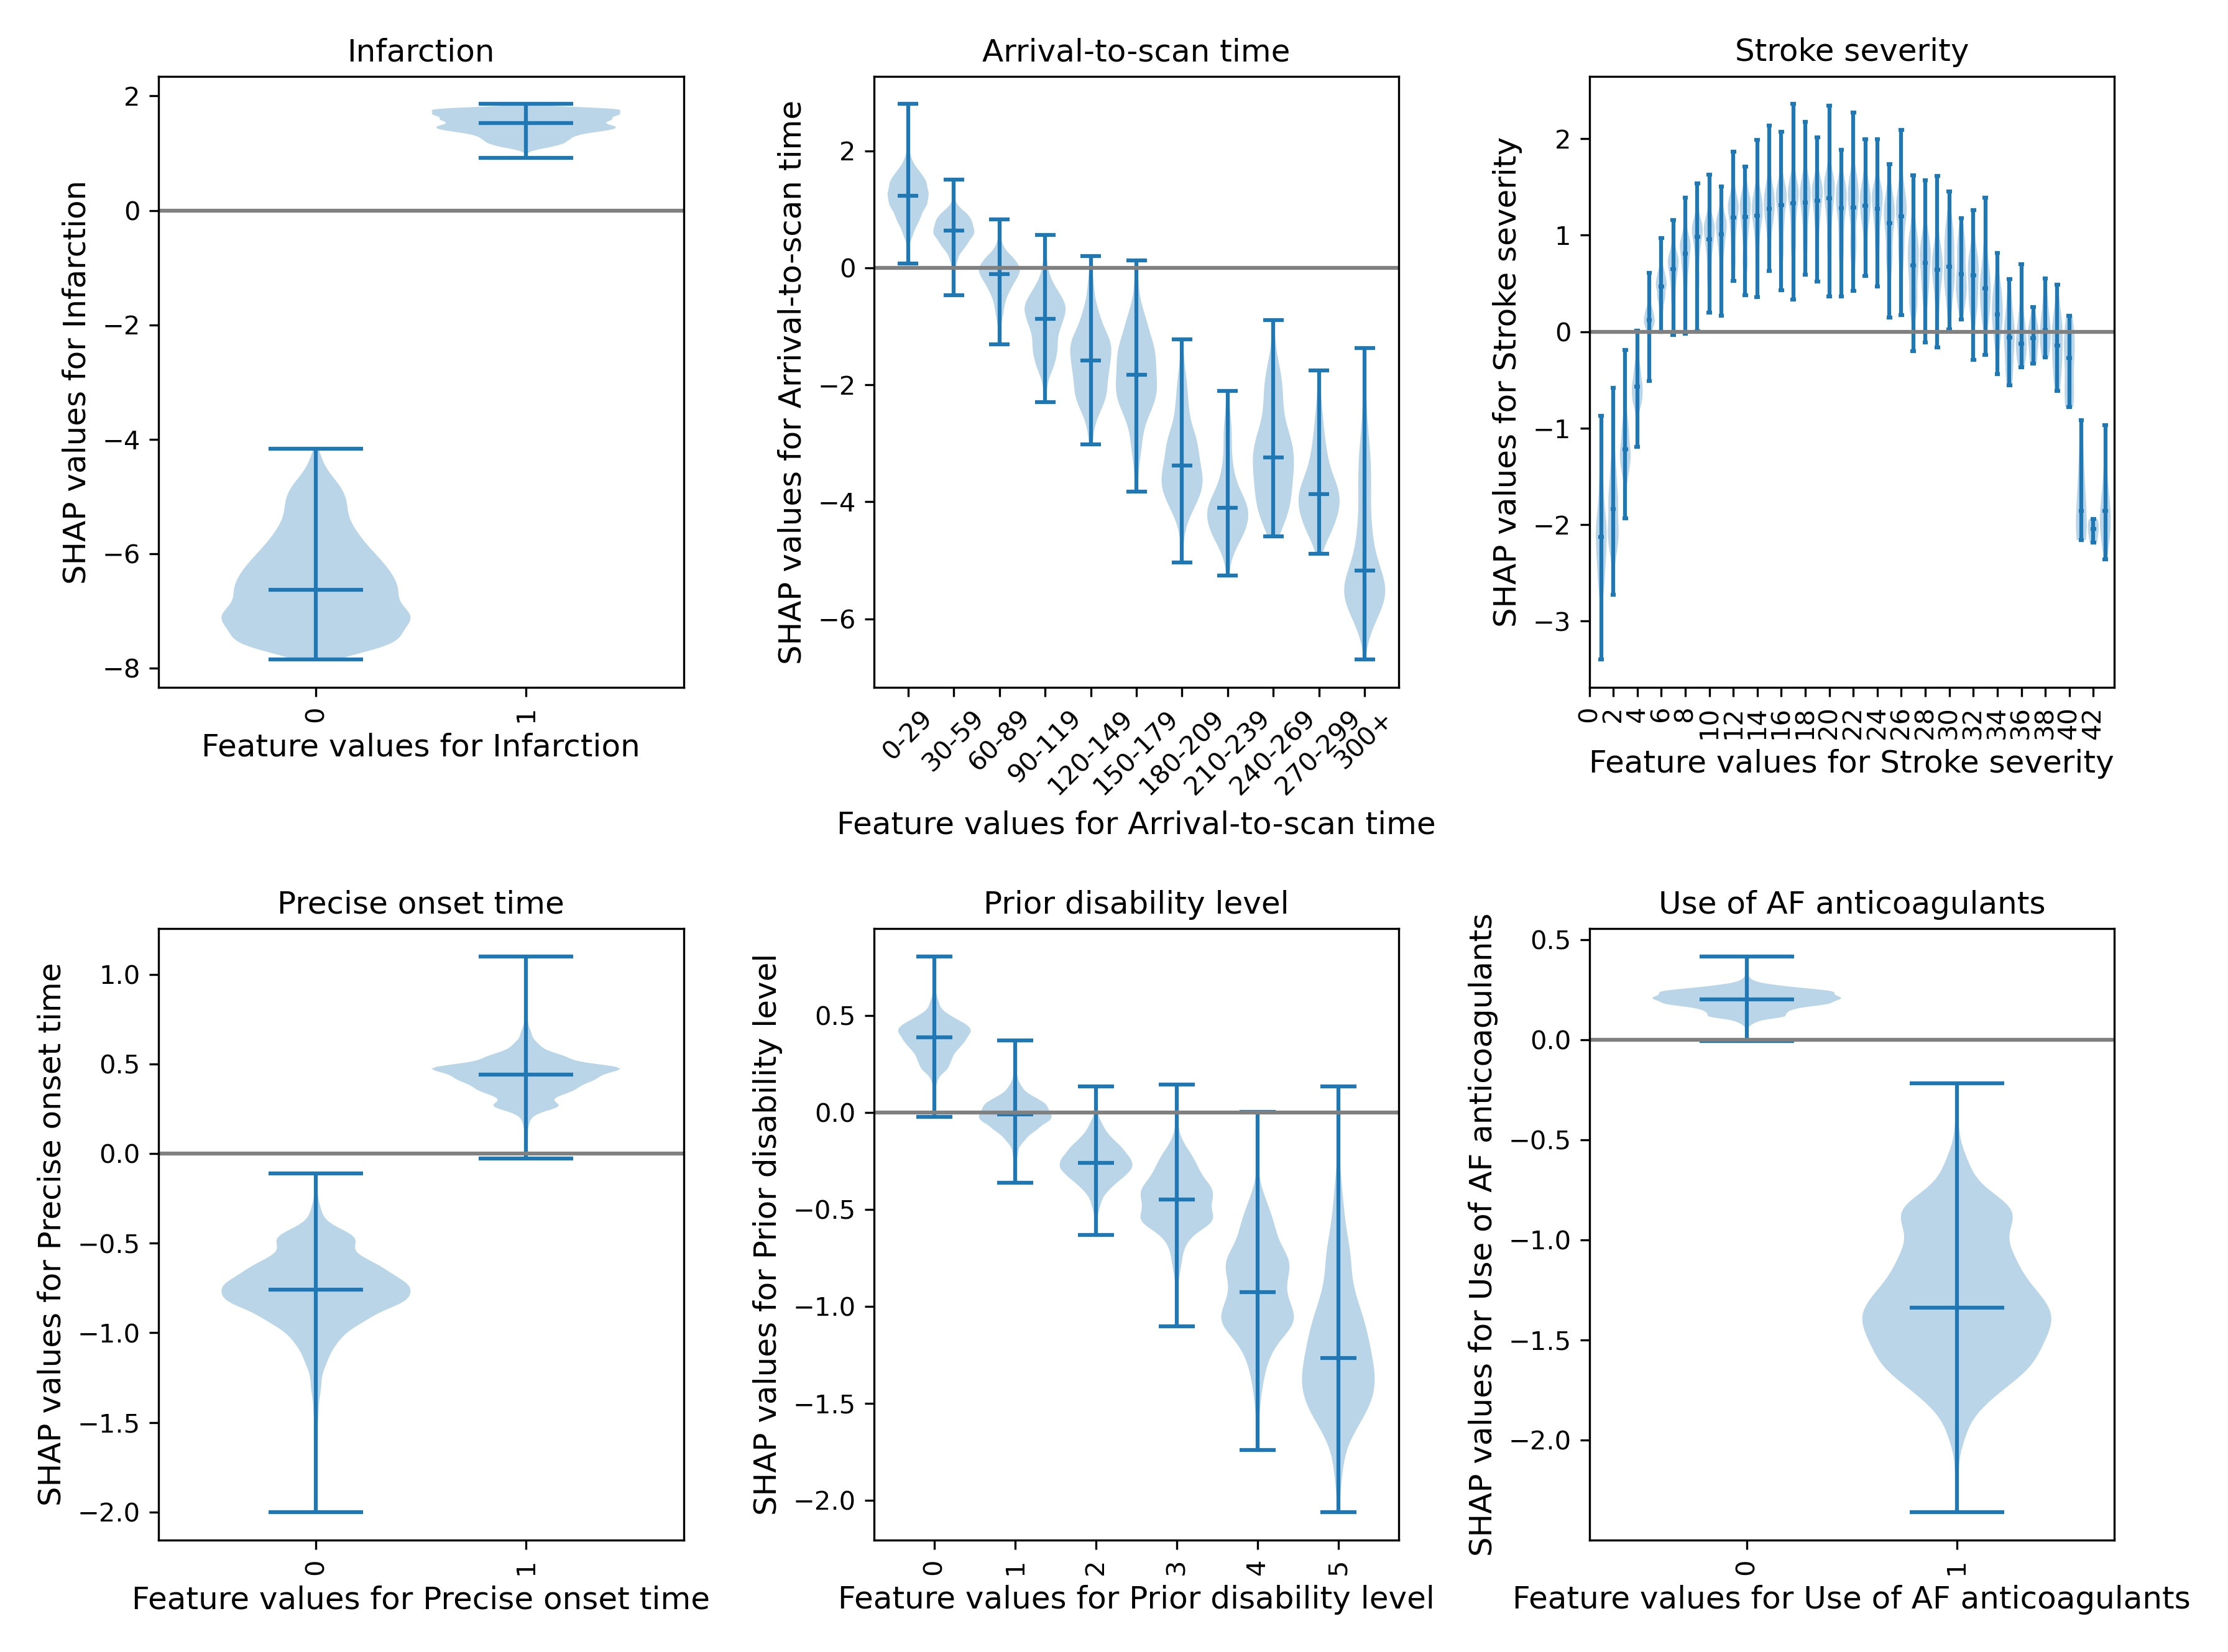
\includegraphics[width=0.78\textwidth]{./images/03_xgb_10_features_thrombolysis_shap_violin}
\end{center}
\end{frame}




%%%%%%%%%%%%%%%%%%%%%%%%%%%%%%%%%%%%%%%%%%%%%%%%%%%%%%%%%%%%%%%

\begin{frame}
\frametitle{Artificial patients}

We can \emph{construct} artificial patients:
\vspace{1mm}
\begin{footnotesize}
\begin{itemize}
    \item Arrival-to-scan time = 15 minutes 
    \item Stroke type  = Infarction
    \item Stroke severity (NIHSS) = 15
    \item Precise onset time = Yes
    \item Prior disability level = None
    \item Use of AF anticoagulants = No
    \item Onset-to-arrival time = 60 minutes
    \item Onset during sleep = No
    \item Age = 72
\end{itemize}
\end{footnotesize}

\vspace{2mm}

99\% hospitals would be expected to give this patient thrombolysis.

\vspace{2mm}

If we change stroke severity to mild (NIHSS), and make the stroke onset time not precise, 35\% hospitals would be expected to give this patient thrombolysis.

\end{frame}

\begin{frame}{Summary (generated by AI*)}

This study used an explainable machine learning model to analyze data from 88,928 patients who arrived at emergency stroke units in England and Wales within 4 hours of known stroke onset.

\vspace{1mm}

The study found that there is substantial variation in the use of thrombolysis, a treatment for stroke, between hospitals, with rates ranging from 7\% to 49\%.

\vspace{1mm}

The study found that factors such as the amount of time between arrival at the hospital and being scanned, the severity of the stroke, the patient’s pre-existing disability, and whether the stroke onset time was known precisely, influenced the odds of receiving thrombolysis. 

\vspace{1mm}

However, the study found that the majority of the variation in thrombolysis use between hospitals may be explained by differences in the hospitals’ willingness to use the treatment, rather than the characteristics of the patients they treated.

\vspace{2mm}
\footnotesize
*Summary generated by ChatGPT (\url{https://openai.com/blog/chatgpt/}).

\end{frame}

\end{document}

